\chapter{Analysis of Receiver Architectures}
\label{chap:rx}



A wide variety of different receiver designs exists each with it's advantages
and drawbacks. To come up with an optimal design, different receiver designs
were investigated using theoretical considerations. Some were simulated to
get an even deeper understanding.
Thereby the focal point was on architectures we could
build in hardware using the Sivers IMA 58-63 GHz converter described in
\secref{sec:comp_sivers}. \\

\section{Transmitter Architecture}
During this report always the same transmitter architecture was used.
It consists of a two channel \gls{DAC} generating the real and imaginary
part of an analytic signal width a bandwidth $B = 1.8 \text{GHz}$
on an \gls{IF} $f_{\text{TX IF}}$. \\

This two signals are than up-converter to
\gls{RF} and a $90^\circ$ coupler is used to suppress the \gls{TX} \gls{LSBand}
as good as possible as described in \secref{sec:rx_rf_1}.
Therefor the \gls{TX} \gls{USBand} is considered the desired signal and the
residual \gls{TX} \gls{LSBand} an interferer. \\

In the following chapters the terms \gls{TX} \gls{USBand} and \gls{TX}
\gls{LSBand} refer to the fact that the up-mixer used for transmitting
produces two signals at $f_{\text{TX LO}} \pm f_{\text{TX IF}}$ where
$f_{\text{TX LO}}$ is the frequency of the transmitter's \gls{LO}
used by the mixer mixing up to \gls{RF}. $f_{\text{TX IF}}$ is the central
frequency of the transmitters \gls{IF} signal. During all experiments
\gls{TX} \gls{USBand} was considered the desired signal and \gls{TX}
\gls{LSBand} a residual signal. \\

Analogous \gls{RX} \gls{USBand} and \gls{RX} \gls{LSBand} refer to
the down-mixer converting energy from $f_{\text{RX LO}} \pm f_{\text{RX IF}}$
to the same receiver \gls{IF} $f_{\text{RX IF}}$. \\

It was measured that in our setup the \gls{TX} \gls{LO} leakage
to the output \gls{RF} signal has similar power than the desired
signal. Therefor this leakage has to be considered as it is a very narrow band,
but high power interferer.
By choosing $f_{\text{TX IF}} = f_{\text{c}} - f_{\text{TX LO}}$ accordingly,
this strong signal can be placed such that it is well suppressed by the channel
filter. \\

Even though setting $f_{\text{TX LO}} = f_{\text{RX LO}}$
would solve the problem of the the suppression of the
undesired \gls{TX} \gls{LO} leakage, in all receivers
$f_{\text{TX LO}}$ and $f_{\text{RX LO}}$ were chosen differently.
This was done to make sure that the residual \gls{TX} \gls{LSBand}
signal does not align with the desired \gls{TX} \gls{USBand} after
down-mixing. A perfect alignment could result in an even better
\gls{SNR} due to the fact that additional signal energy is transmitted
alongside the desired \gls{TX} \gls{USBand} signal in an other channel.
This must not be done according to relevant standards. \\

\section{RF Architecture}
When building a receiver, one faces the problem of isolating the channel of
interest from all others signals received by the antenna. Therefor
two ways of building channel selection filters are discussed in the following
chapters. \\

All receivers have a band filter directly after the antenna simply by the
fact that all components (antenna, amplifiers, mixers etc.) have a frequency
selectivity which is typically optimized for the band of interest only.
An additional band filter might be added to minimize the total power supplied
to the \gls{LNA} which has the main influence of the total noise figure of
the receiver. \\

Inside this band there are typically multiple channels with a carrier frequency
$f_c$ and a bandwidth $B$. \\

Since it is hard to build adjustable filters on \gls{RF} to select one specific
channel, this selection is typically done on an \acrfull{IF}. In our case of a
carrier frequency of $f_c \approx 60 \;\text{GHz}$ this \gls{IF}
is always lower than the carrier frequency $f_c$ due to component restrictions. \\

\subsection{Image Rejection using High Intermediate Frequency}
\label{sec:rx_rf_0}
First we look at the architecture shown in \figref{fig:rx_rf_0_bd} where
the mixer uses a \gls{LO} at $f_{\text{RX LO}}$ to mix the signal $s(t)$
centered around $f_{c}$ to an \gls{IF} signal $i(t)$ at
$f_{\text{RX IF}} = f_{c} - f_{\text{RX LO}}$ as shown in \figref{fig:rx_rf_0_freq_s}
and \figref{fig:rx_rf_0_freq_i}. \\

This mixer produces a total of four signal components:
\begin{align}
  + f_{c} + f_{\text{RX LO}} \\
  + f_{c} - f_{\text{RX LO}} \\
  - f_{c} + f_{\text{RX LO}} \\
  - f_{c} - f_{\text{RX LO}}
\end{align}

The two signals $\pm (f_{c} + f_{\text{RX LO}})$ are not relevant since their
frequency is above 100 GHz and well beyond what the mixer output can drive. \\

When $f_{\text{RX IF}}$ is high enough, the undesired \gls{RX} \gls{LSBand}
signal at $-f_{\text{c}} + f_{\text{RX LO}}$ lies outside the band filter
and therefor is zero. Otherwise it would convolve with the desired
\gls{RX} \gls{USBand} signal. This leads to a lower bound
$f_{\text{RX IF}} \geq B$ for the \gls{RX} \gls{IF} frequency
\footnote{%
  In fact $f_{\text{RX IF}} \geq \frac{B}{2}$
  is sufficient if later stages of the receiver can switch
  between \gls{USBand} and \gls{LSBand} reception and
  $f_{\text{RX LO}}$ is chosen to be at the lower or upper edge of the
  channel filter accordingly.}. \\

A fixed channel filter is than used to suppress neighbouring channels. \\

\begin{figure}[p]
  \centering
  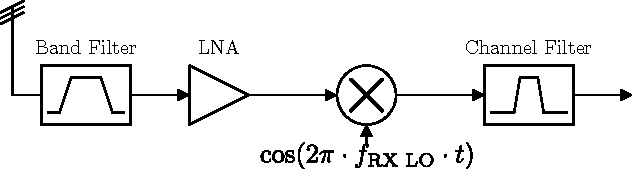
\includegraphics[width=0.7\textwidth]{figures/rx_rf_0_bd}
  \caption{Block Diagram of Image Rejection using high \gls{IF}}
  \label{fig:rx_rf_0_bd}
\end{figure}

\begin{figure}[p]
  \centering
  \begin{subfigure}{\textwidth}
    \centering
    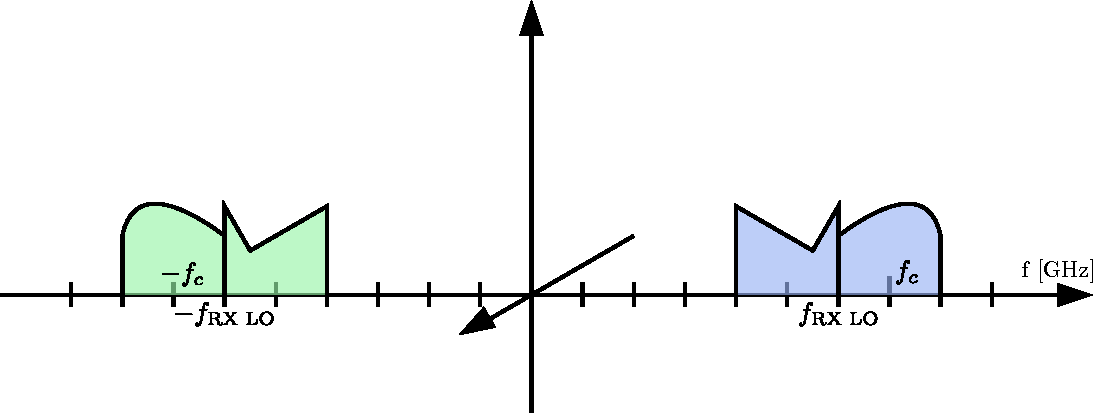
\includegraphics[width=0.8\textwidth]{figures/rx_rf_0_freq_s}
    \caption{$s(t)$}
    \label{fig:rx_rf_0_freq_s}
  \end{subfigure}
  \vspace{4ex} \\
  \begin{subfigure}{\textwidth}
    \centering
    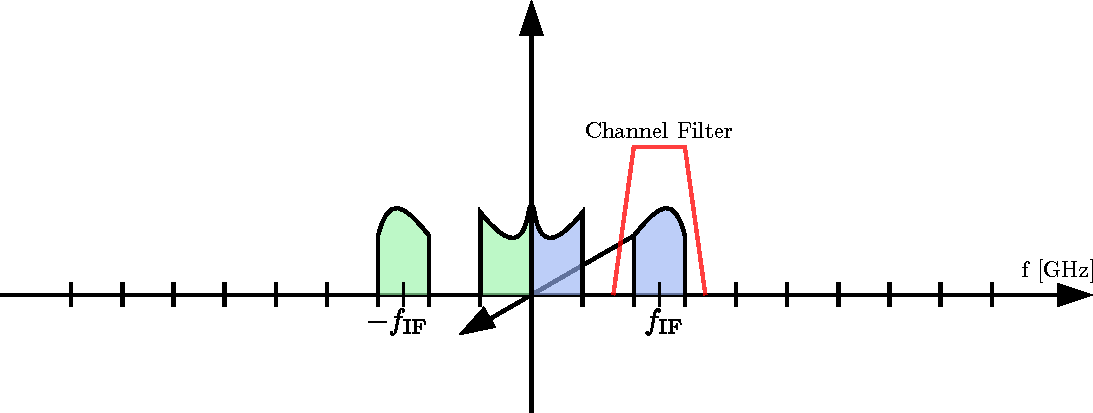
\includegraphics[width=0.8\textwidth]{figures/rx_rf_0_freq_i}
    \caption{$i(t)$}
    \label{fig:rx_rf_0_freq_i}
  \end{subfigure}
  \caption{Image Rejection using High Intermediate Frequency}
  \label{fig:rx_rf_0_freq}
\end{figure}

\subsection{Image Rejection using $90^\circ$ Couplers}
\label{sec:rx_rf_1}
The use of a high \gls{IF}, as described in the last section, might
by very favorable for short wave receivers where the band filters
are narrow (a few MHz) and the \gls{IF} is typically between 10 and 100 MHz.
For 60 GHz applications, where band filters are approximately 5GHz wide,
an \gls{IF} of a few GHz is required.
Therefor a more suitable way to do channel selection is described in this
section. \\

The suppression of the undesired \gls{RX} \gls{LSBand} signal can also be done
using a $90^\circ$ couplers as described in \secref{sec:comp_90deg}: \\

Let us assume, that we have the real \gls{RF} signal $r(t)$ shown in
\figref{fig:rx_rf_1_freq_s}.
The blue round signal centered around the carrier frequency $+f_c$ is our
desired signal laying in the \gls{USBand} of the \gls{RX} mixer.
The spiky signal is a neighbouring channel laying exactly
where the \gls{LSBand} of the \gls{RX} mixer is and therefor has to
be suppressed.
Since it is a real signal, the negative frequencies consist of the mirrored,
complex conjugate signals which are painted in green. \\

By splitting $r(t)$ using a $90^\circ$ coupler we obtain the two signals
$r(t)$ and $\mathcal{H}^{-1}\{r(t)\}$ (drawn in \figref{fig:rx_rf_1_freq_Hs}).
$\mathcal{H}^{-1}$ denotes the inverse Hilbert transform which rotates the phase
of a signal by $j$ for positive and $-j$ for negative frequencies.
The transfer function of the Hilbert transform is shown in
\figref{fig:hilbert}. \\

Next both signals are mixed by $f_{\text{RX LO}}$ resulting in two new signals
$a(t)$ and $b(t)$ as shown in \figref{fig:rx_rf_1_freq_a} and
\figref{fig:rx_rf_1_freq_b}.
The high mirror signals at $\pm (f_c + f_{\text{RX LO}})$ are already
ignored. \\

By using a second $90^\circ$ coupler that applies the Hilbert transform
to $b(t)$ (drawn in \figref{fig:rx_rf_1_freq_Hb})
and adds $a(t)$ we end up with the real signal
$c(t) = a(t) + \mathcal{H}\{b(t)\}$
which is shown in \figref{fig:rx_rf_1_freq_c}.
As we can see, all signals with a lower frequency than $f_{\text{RX LO}}$
cancel out, while those with a higher frequency than $f_{\text{RX LO}}$
positively interfere. \\

One should note that the difference between $\mathcal{H}$ and $\mathcal{H}^{-1}$
is simply a swap of the two output plugs of a $90^\circ$ coupler since
the absolute phase rotation can be considered to be part of the channel.
In fact both outputs are delayed in time corresponding to negative phase
rotation for positive frequencies and a positive phase rotation for negative
frequencies. \\

Finally a fixed channel selection filter can be used at an arbitrary \gls{IF}
which is a clear advantage over the method discussed in \secref{sec:rx_rf_0}. \\

\begin{figure}[h!]
  \centering
  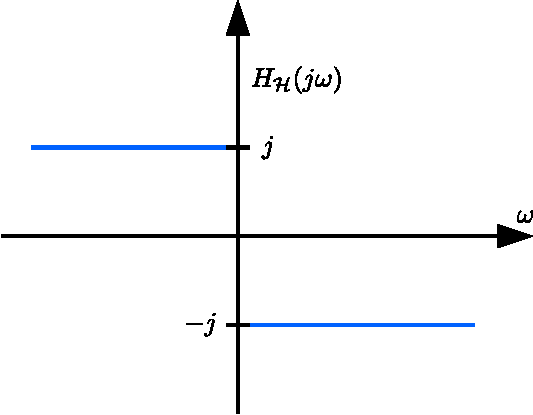
\includegraphics[width=0.3\textwidth]{figures/hilbert}
  \caption{Transfer Function of Hilbert Transform}
  \label{fig:hilbert}
\end{figure}

\begin{figure}[p]
  \centering
  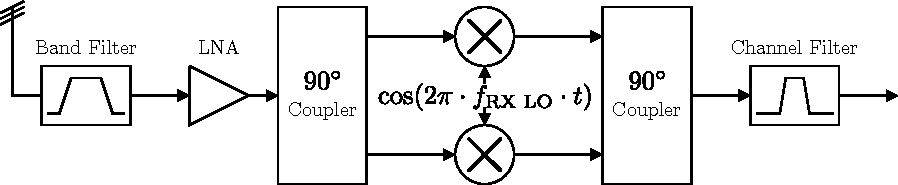
\includegraphics[width=\textwidth]{figures/rx_rf_1_bd}
  \caption{Block Diagram of Image Rejection using $90^\circ$ Couplers}
  \label{fig:rx_rf_1_bd}
\end{figure}

\begin{figure}[p]
  \centering
  \begin{subfigure}{0.45\textwidth}
    \centering
    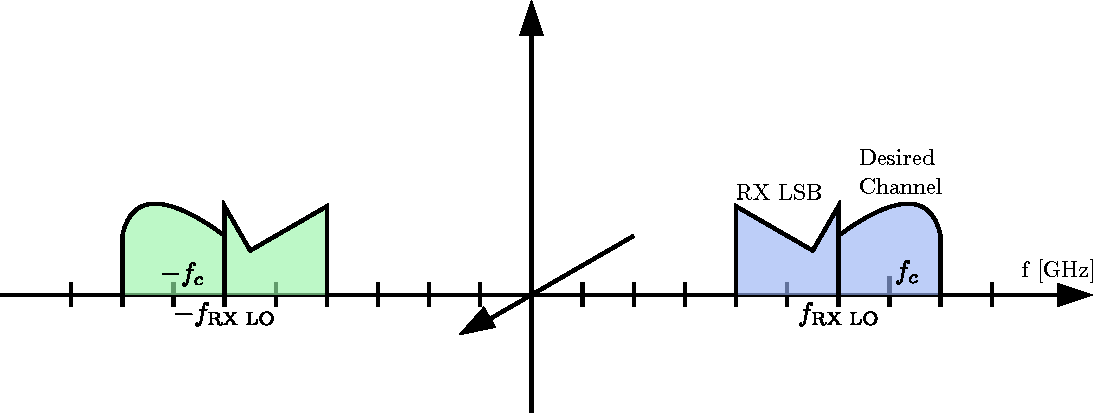
\includegraphics[width=\textwidth]{figures/rx_rf_1_freq_s}
    \caption{$r(t)$}
    \label{fig:rx_rf_1_freq_s}
  \end{subfigure}
  ~
  \begin{subfigure}{0.45\textwidth}
    \centering
    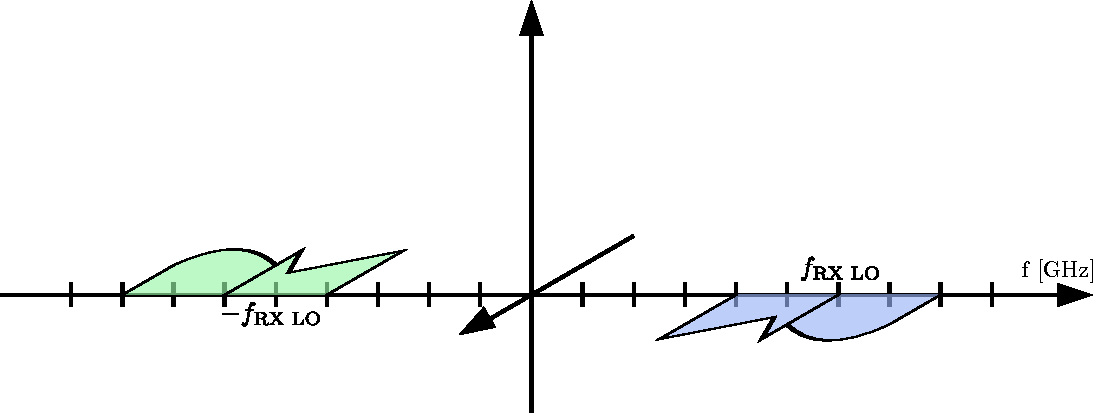
\includegraphics[width=\textwidth]{figures/rx_rf_1_freq_Hs}
    \caption{$\mathcal{H}^{-1}\{r(t)\}$}
    \label{fig:rx_rf_1_freq_Hs}
  \end{subfigure}
  \vspace{4ex} \\
  \begin{subfigure}{0.45\textwidth}
    \centering
    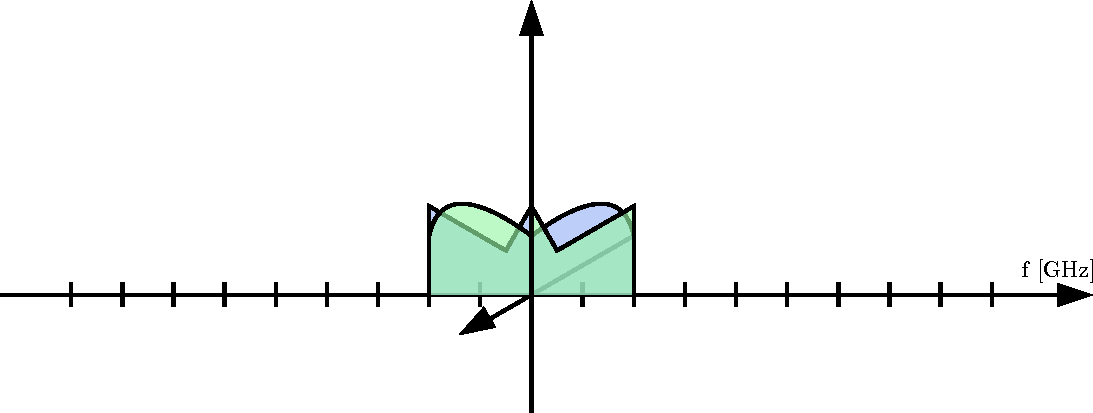
\includegraphics[width=\textwidth]{figures/rx_rf_1_freq_a}
    \caption{$a(t)$}
    \label{fig:rx_rf_1_freq_a}
  \end{subfigure}
  ~
  \begin{subfigure}{0.45\textwidth}
    \centering
    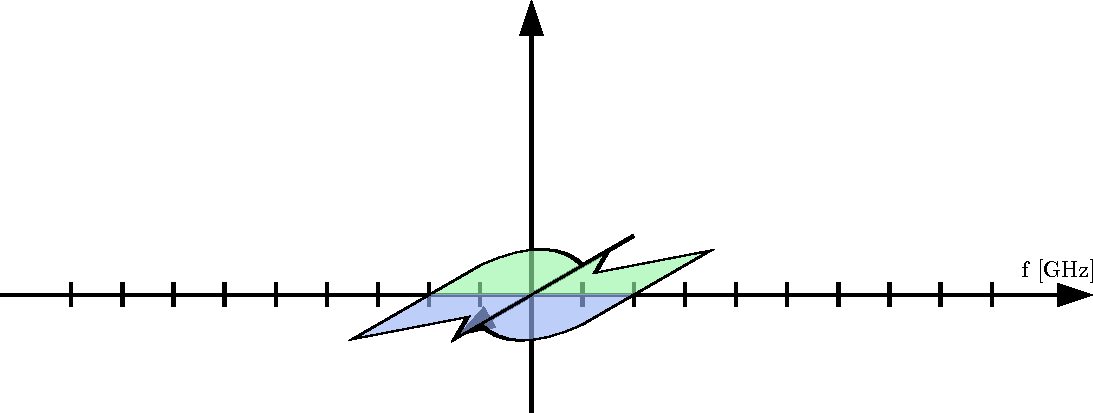
\includegraphics[width=\textwidth]{figures/rx_rf_1_freq_b}
    \caption{$b(t)$}
    \label{fig:rx_rf_1_freq_b}
  \end{subfigure}
  \vspace{4ex} \\
  \begin{subfigure}{0.45\textwidth}
    \centering
    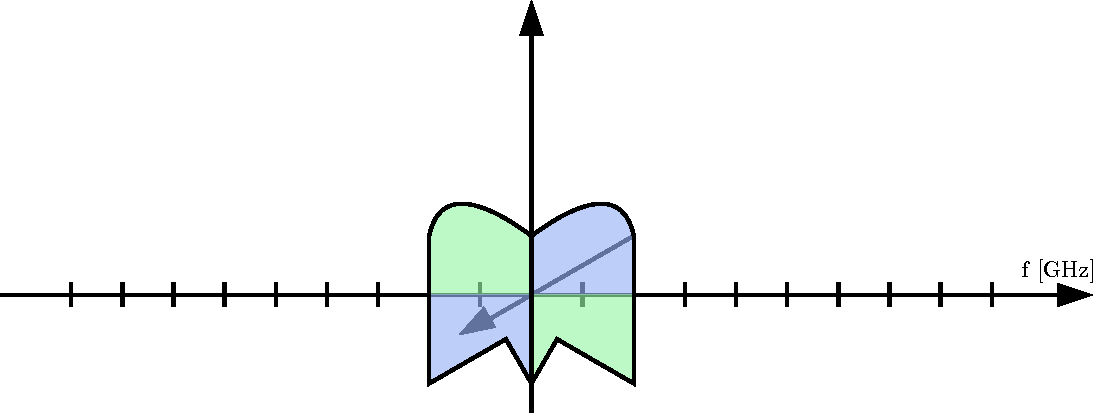
\includegraphics[width=\textwidth]{figures/rx_rf_1_freq_Hb}
    \caption{$\mathcal{H}^{-1}\{b(t)\}$}
    \label{fig:rx_rf_1_freq_Hb}
  \end{subfigure}
  ~
  \begin{subfigure}{0.45\textwidth}
    \centering
    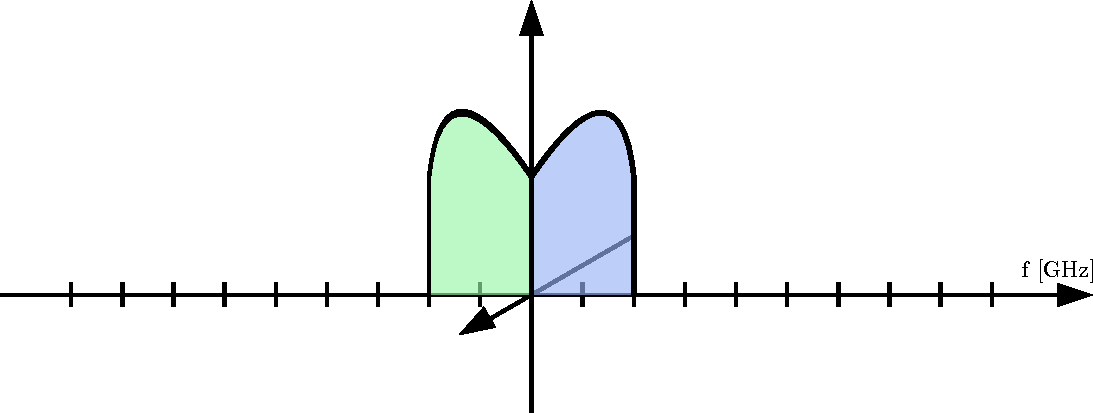
\includegraphics[width=\textwidth]{figures/rx_rf_1_freq_c}
    \caption{$c(t) = a(t) + \mathcal{H}^{-1}\{b(t)\}$}
    \label{fig:rx_rf_1_freq_c}
  \end{subfigure}
  \caption{Image Rejection using $90^\circ$ Couplers}
  \label{fig:rx_rf_1_freq}
\end{figure}

\section{IF Architecture}
After the \gls{RF} part did the channel selection only the desired signal
is left and should be digitized.
This can be accomplished using different
mixing schemes of which three are shown in this section. \\

\subsection{Quadrature Baseband Sampling}
\label{sec:rx_adc_1}
The first \gls{IF}, which was previously used for the channel selection filter,
can be directly converted to baseband by a second mixer with
$f_{\text{LO}_2} = f_{\text{IF}}$.
Since our signal is asymmetric, the baseband signal is not analytic
and therefor quadrature sampling, which uses two mixers as shown in
\figref{fig:rx_adc_1_bd}, can be used. \\

Considering an \gls{IF} signal $i(t)$ with a center frequency of
$f_{\text{IF RX}}$ and using the transformation \eqref{eq:four_cos},
we can plot $i(t)$ mixed with $\cos(2\pi \cdot f_{\text{IF}} \cdot t)$.
See \figref{fig:rx_adc_1_freq_s}, \figref{fig:rx_adc_1_freq_cos}
and \figref{fig:rx_adc_1_freq_a}. \\

Analogous using \eqref{eq:four_sin} can be used to draw $i(t)$ mixed with
$\sin(2\pi \cdot f_{\text{IF}} \cdot t)$.
See \figref{fig:rx_adc_1_freq_sin} and \figref{fig:rx_adc_1_freq_b}. \\

\begin{align}
  \cos(\omega_0 \cdot t) \;\; & \laplace \;\; \pi
  \left[\delta(\omega - \omega_0) + \delta(\omega + \omega_0) \right]
  \label{eq:four_cos} \\
  \sin(\omega_0 \cdot t) \;\; & \laplace \;\; \frac{\pi j}{2}
  \left[\delta(\omega + \omega_0) - \delta(\omega - \omega_0) \right]
  \label{eq:four_sin}
\end{align}

$a(t)$ and $b(t)$ are than low pass filtered to suppress the mirror image
at $2 f_{\text{IF}}$ and sampled by a two channel \gls{ADC} running with a
sample rate $f_s \geq B$. \\

Next the analytic signal $c(t)$ is constructed without any calculations
by simply interpreting the \gls{ADC} channels as
$c(t) = b(t) + j \cdot a(t)$. To show that this works $j \cdot a(t)$
is plotted in \figref{fig:rx_adc_1_freq_ja} and
$c(t)$ in \figref{fig:rx_adc_1_freq_c}.

\begin{figure}[p]
  \centering
  \begin{subfigure}{0.45\textwidth}
    \centering
    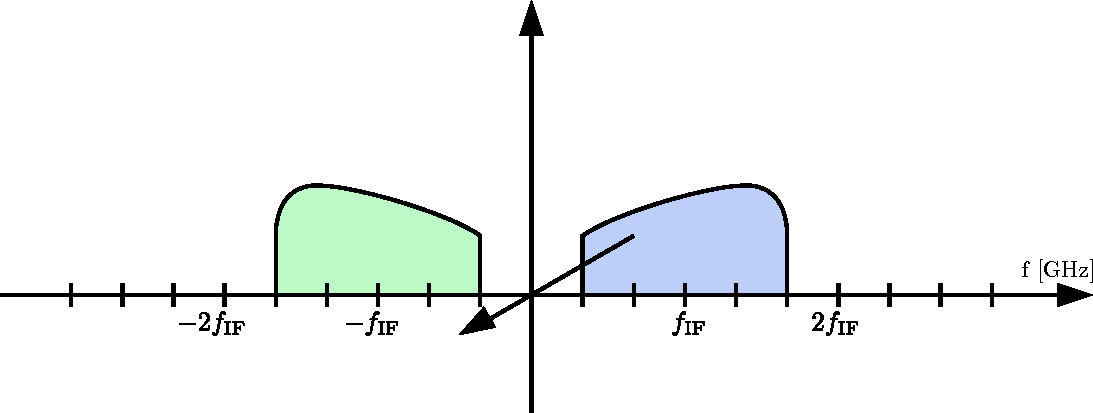
\includegraphics[width=\textwidth]{figures/rx_adc_1_freq_i}
    \caption{$i(t)$}
    \label{fig:rx_adc_1_freq_s}
  \end{subfigure}
  \vspace{4ex} \\
  \begin{subfigure}{0.45\textwidth}
    \centering
    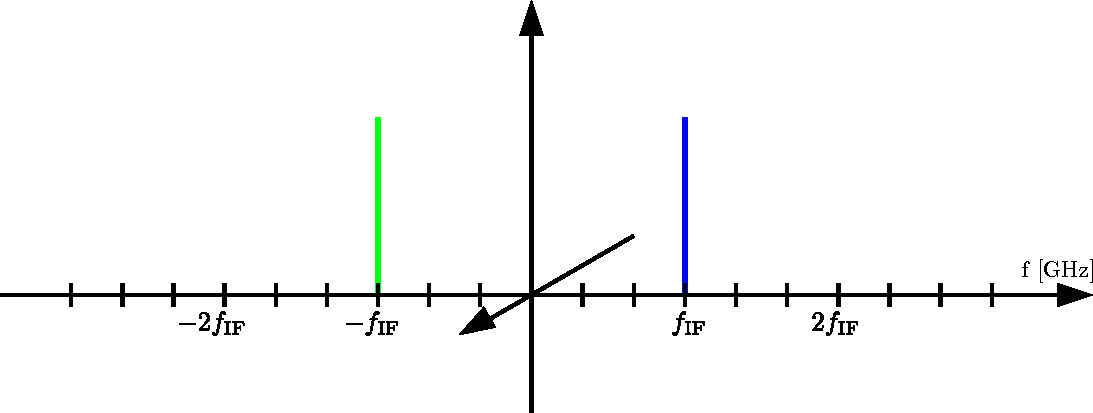
\includegraphics[width=\textwidth]{figures/rx_adc_1_freq_cos}
    \caption{$\cos(2\pi \cdot f_{\text{IF}} \cdot t)$}
    \label{fig:rx_adc_1_freq_cos}
  \end{subfigure}
  ~
  \begin{subfigure}{0.45\textwidth}
    \centering
    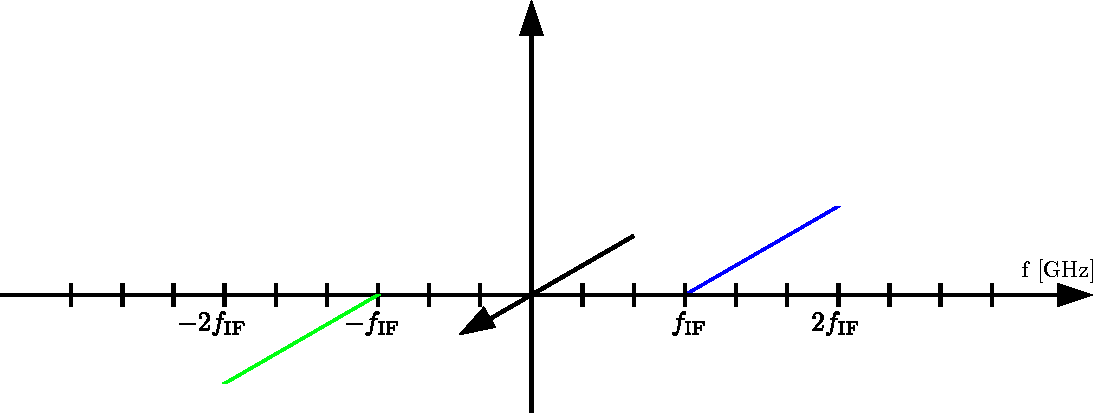
\includegraphics[width=\textwidth]{figures/rx_adc_1_freq_sin}
    \caption{$\sin(2\pi \cdot f_{\text{IF}} \cdot t)$}
    \label{fig:rx_adc_1_freq_sin}
  \end{subfigure}
  \vspace{4ex} \\
  \begin{subfigure}{0.45\textwidth}
    \centering
    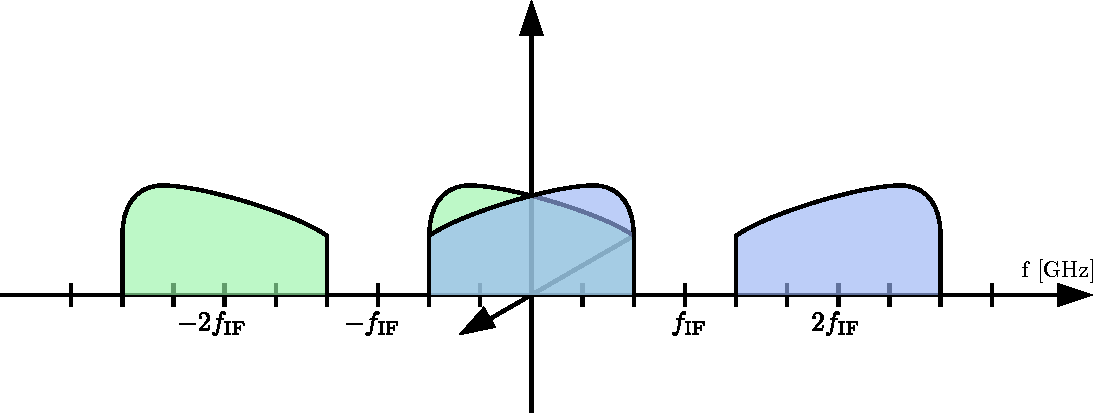
\includegraphics[width=\textwidth]{figures/rx_adc_1_freq_a}
    \caption{$a(t) = i(t) \cdot \cos(2\pi \cdot f_{\text{IF}} \cdot t)$}
    \label{fig:rx_adc_1_freq_a}
  \end{subfigure}
  ~
  \begin{subfigure}{0.45\textwidth}
    \centering
    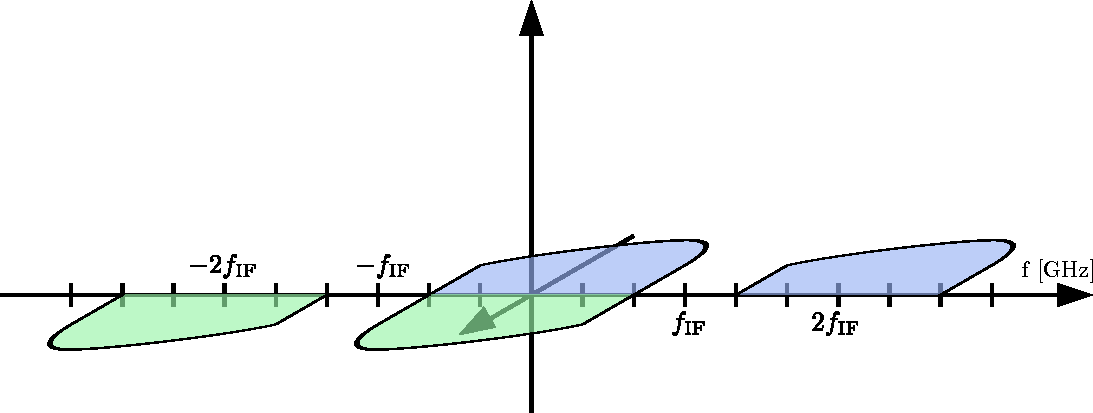
\includegraphics[width=\textwidth]{figures/rx_adc_1_freq_b}
    \caption{$b(t) = i(t) \cdot \sin(2\pi \cdot f_{\text{IF}} \cdot t)$}
    \label{fig:rx_adc_1_freq_b}
  \end{subfigure}
  \vspace{4ex} \\
  \begin{subfigure}{0.45\textwidth}
    \centering
    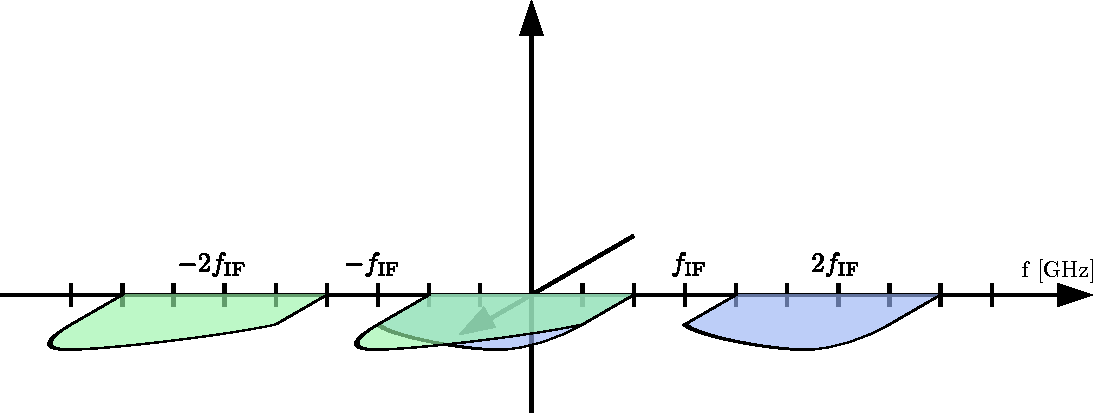
\includegraphics[width=\textwidth]{figures/rx_adc_1_freq_ja}
    \caption{$j \cdot a(t)$}
    \label{fig:rx_adc_1_freq_ja}
  \end{subfigure}
  ~
  \begin{subfigure}{0.45\textwidth}
    \centering
    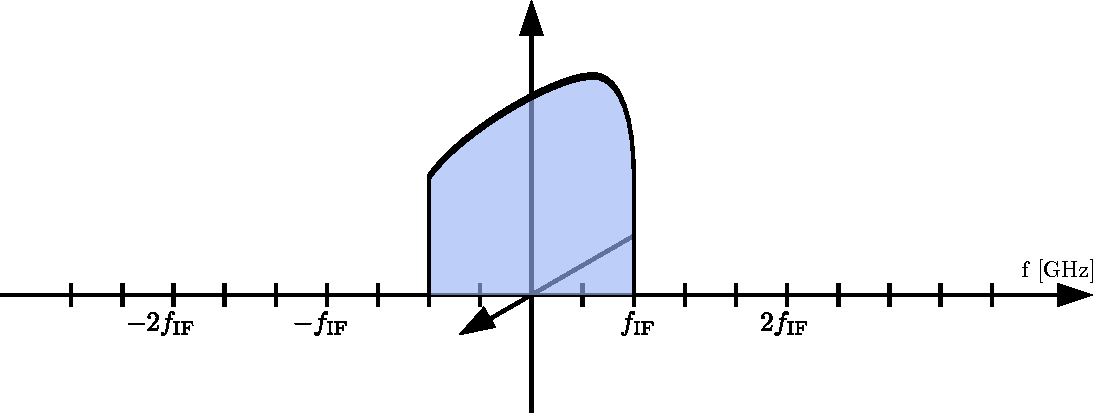
\includegraphics[width=\textwidth]{figures/rx_adc_1_freq_c}
    \caption{$c(t) = \text{LP}\{b(t)\} + j \text{LP}\{\cdot a(t)\}$}
    \label{fig:rx_adc_1_freq_c}
  \end{subfigure}
  \caption{Quadrature Baseband Mixing}
  \label{fig:rx_adc_1_freq}
\end{figure}

\begin{figure}[p]
  \centering
  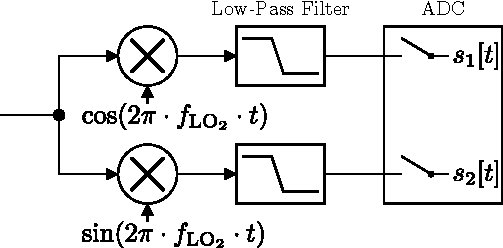
\includegraphics[width=0.7\textwidth]{figures/rx_adc_1_bd}
  \caption{Block Diagram of Quadrature Baseband Sampling Receiver}
  \label{fig:rx_adc_1_bd}
\end{figure}

\subsection{First Nyquist-Zone Sampling}
\label{sec:rx_adc_0}
Instead of using two \gls{ADC} channels, the signal can also be mixed
to the first Nyquist-zone $[0 \; \frac{f_s}{2}]$ and sampled by just one
channel. \\

This results in a second \gls{IF} of $f_{\text{LO}_2} = \frac{f_s}{2}$ where
the sample rate $f_s$ has to be at least double the bandwidth $B$:
\[f_s \geq 2 \cdot B\]

Therefor the 1.8 GHz wide signal fully falls into the first Nyquist-zone of
a single \gls{ADC} sampling at 3.6 GHz. Again a \gls{DC}-block
is used in front of the \gls{ADC}. Compared to the Quadrature Baseband
Sampling Receiver only half of the signal is lost this time since
the \gls{DC}-block now deletes the lowest frequency part of the signal
and not the central part symmetrically around zero. Also this error
can be completely avoided by using a bandwidth $B$ slightly lower than
$\frac{f_s}{2}$. \\

\begin{figure}[p]
  \centering
  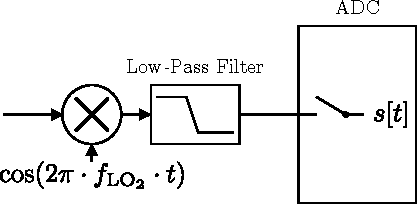
\includegraphics[width=0.7\textwidth]{figures/rx_adc_0_bd}
  \caption{Block Diagram of First Nyquist-Zone Sampling Receiver}
  \label{fig:rx_adc_0_bd}
\end{figure}

\subsection{Quadrature Sub-Nyquist Sampling}
\label{sec:rx_adc_2}
Typically, a low-pass filter before the \gls{ADC} makes sure, that only
signals below $\frac{f_s}{2}$ are supplied to the sample and hold circuit
of the \gls{ADC} in order to avoid aliasing.
$\frac{f_s}{2}$ is therefor the digital bandwidth of an \gls{ADC}. \\

However, an \gls{ADC} can have a bigger analog bandwidth. This means that
even faster signals are correctly captures by the sample and hold circuit
at the input of the \gls{ADC}. The frequency space between 0 and
$\frac{f_s}{2}$ is often referred to as first Nyquist-zone as shown in
\figref{fig:rx_adc_2_nyquist_zones}. \\
The frequency space between $\frac{f_s}{2}$ and $f_s$ is referred to as
second Nyquist-zone and so on. After sampling a signal, all energy captured
in the second Nyquist-zone wraps at $\frac{f_s}{2}$ and adds up with the energy
in the first Nyquist-zone.
By making sure, that no significant signal energy overlaps, no information%
\footnote{except the information in which Nyquist-zone the signal was before
  sampling} is lost. \\

This trick can be combined with the Quadrature Baseband Sampling described
in \secref{sec:rx_adc_1} to capture a total bandwidth of
$B = 2 \cdot \frac{f_s}{2}$ with two \gls{ADC} channels sampling at $f_s$ each. \\

\begin{figure}[p]
  \centering
  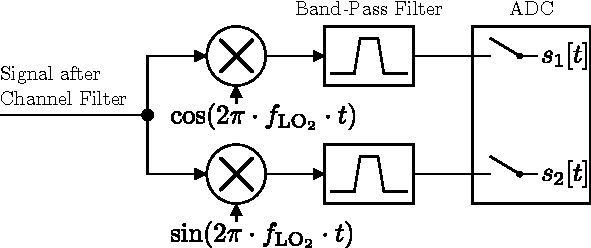
\includegraphics[width=0.7\textwidth]{figures/rx_adc_2_bd}
  \caption{Block Diagram of Quadrature Sub-Nyquist Sampling Receiver}
  \label{fig:rx_adc_2_bd}
\end{figure}

\begin{figure}[p]
  \centering
  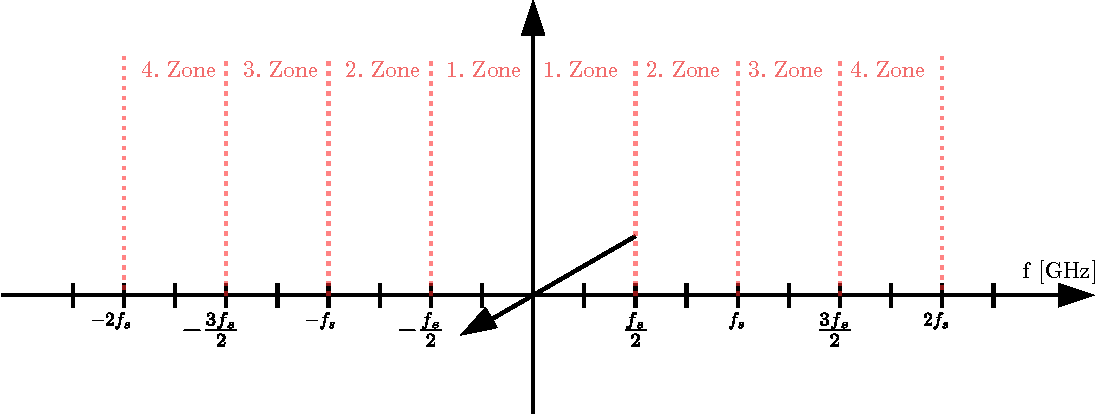
\includegraphics[width=0.7\textwidth]{figures/rx_adc_2_nyquist_zones}
  \caption{Nyquist-Zones}
  \label{fig:rx_adc_2_nyquist_zones}
\end{figure}

\section{Evaluation of Complete Receiver Architectures}
To implement a complete receiver, the first part of doing the channel selection,
and the second part responsible for digitizing the signal have do be combined. \\

The following sections cover three different architectures. Whenever possible,
example frequencies are given that are supported by the hardware described in
\chapref{chap:comp}. Also their advantages and drawbacks are discussed. \\

\subsection{Quadrature Baseband Sampling Receiver}
\label{sec:rx_0}
The Quadrature Baseband Sampling Receiver drawn in \figref{fig:rx_0_bd}
is based on the image rejection by a high enough \gls{IF} frequency as
described in \secref{sec:rx_rf_0} and than uses quadrature baseband sampling
as described in \secref{sec:rx_adc_1}.
The used frequencies are listed in \tblref{tab:rx_0} and the spectra are drawn
in \figref{fig:rx_0_freq}. \\

To do the Quadrature Baseband Sampling the
$\cos(2\pi \cdot f_{\text{LO}_2} \cdot t)$ as well as a $90^\circ$
phase shifted version $\sin(2\pi \cdot f_{\text{LO}_2} \cdot t)$ has to be
generated.
The high \gls{IF} of the receiver ($f_{\text{RX IF}} = 5.9 \;\text{GHz}$)
requires the \gls{LO} for the second mixing stage to run at
$f_{\text{LO}_2} = 5.9 \;\text{GHz}$ as well which is out of the, more or less,
linear range of the Meca 3 dB Hybrid Coupler 705S-3.000 described in
\secref{sec:comp_90deg}. Also the $f_{\text{RX IF}}$ does not meet the
specification of the 58-63 GHz converter described in
\secref{sec:comp_sivers}. \\

Self-mixing of the \gls{LO} at $f_{\text{LO}_2}$ of these mixers lead
to a \gls{DC}-offset which has to be blocked in order for the
\glspl{ADC} to work at full range.
Therefor all \glspl{ADC} are always used with \gls{DC}-blocks as described
in \secref{sec:comp_dc_block}. This high-pass filters unfortunately
not only remove \gls{DC} but also a small portion of the signal,
resulting in some \gls{ISI}. \\

\begin{table}[h]
  \centering
  \begin{tabular}{|l|r@{}l@{~}l|}
    \hline
    $f_{\text{TX IF}}$              & 1&.7&GHz \\ \hline
    $f_{\text{TX LO}}$              & 59&.2&GHz \\ \hline
    $f_{\text{RX LO}}$              & 55&&GHz \\ \hline
    $f_{\text{RX IF}}$              & 5&.9&GHz \\ \hline
    $f_{\text{LO}_2}$               & 5&.9&GHz \\ \hline
    $f_c$                         & 60&.9&GHz \\ \hline
    Signal Bandwidth B            & 1&.8&GHz \\ \hline
    Number of \gls{ADC} Channels  & 2 && \\ \hline
    Sample Rate $f_s$ & 1&.8&GHz \\ \hline
  \end{tabular}
  \caption{Properties of Quadrature Baseband Sampling Receiver}
  \label{tab:rx_0}
\end{table}

\begin{figure}[p]
  \centering
  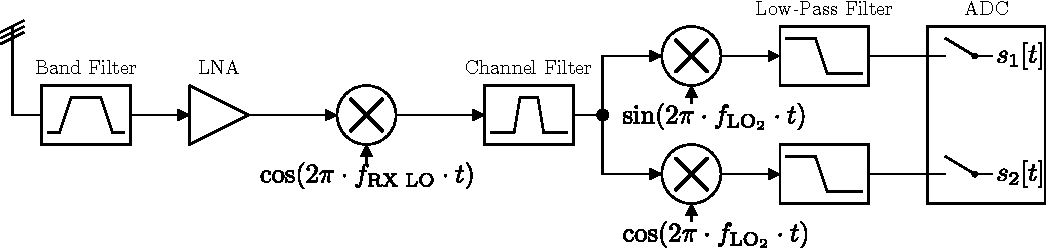
\includegraphics[width=\textwidth]{figures/rx_0_bd}
  \caption{Block Diagram of Quadrature Baseband Sampling Receiver}
  \label{fig:rx_0_bd}
\end{figure}

\begin{figure}[p]
  \centering
  \begin{subfigure}{\textwidth}
    \centering
    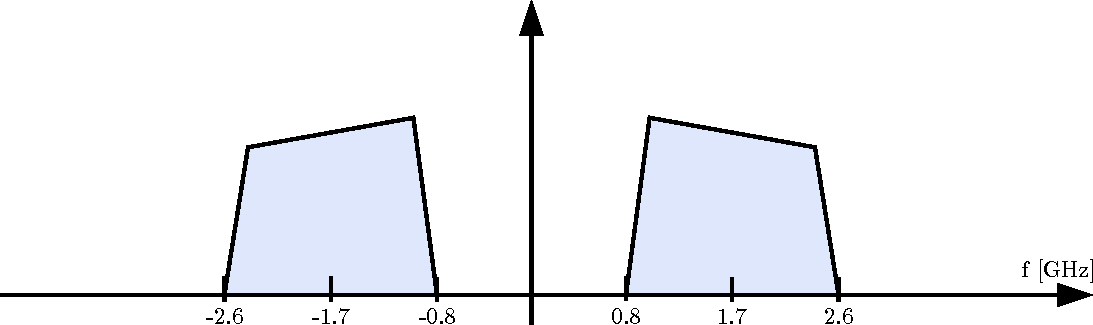
\includegraphics[width=0.8\textwidth]{figures/rx_0_freq_tx_if}
    \caption{\gls{TX} \gls{IF}}
    \label{fig:rx_0_frq_tx_if}
  \end{subfigure}
  \vspace{4ex} \\
  \begin{subfigure}{\textwidth}
    \centering
    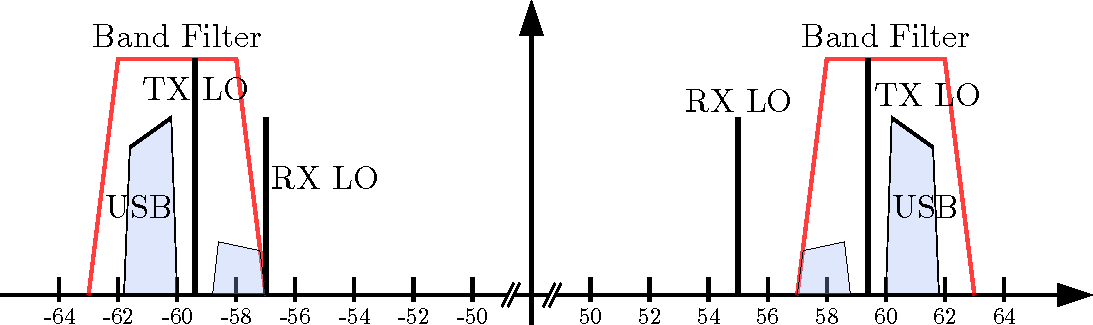
\includegraphics[width=0.8\textwidth]{figures/rx_0_freq_rf}
    \caption{\gls{RF}}
    \label{fig:rx_0_freq_rf}
  \end{subfigure}
  \vspace{4ex} \\
  \begin{subfigure}{\textwidth}
    \centering
    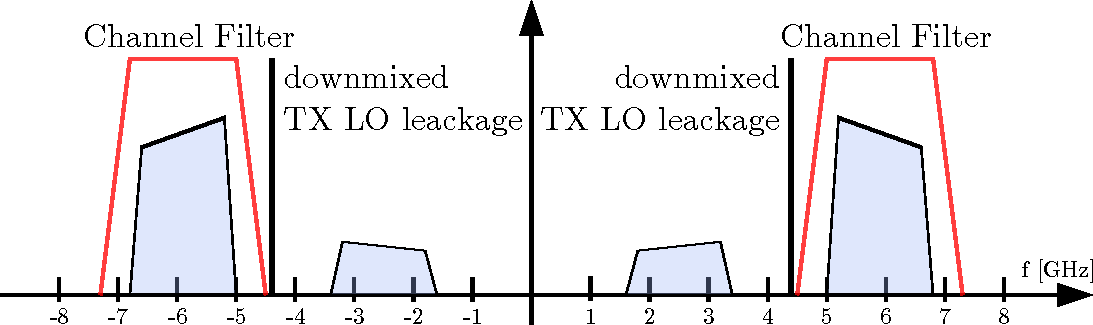
\includegraphics[width=0.8\textwidth]{figures/rx_0_freq_rx_if1}
    \caption{\gls{RX} high \gls{IF}}
    \label{fig:rx_0_freq_rx_if1}
  \end{subfigure}
  \vspace{4ex} \\
  \begin{subfigure}{\textwidth}
    \centering
    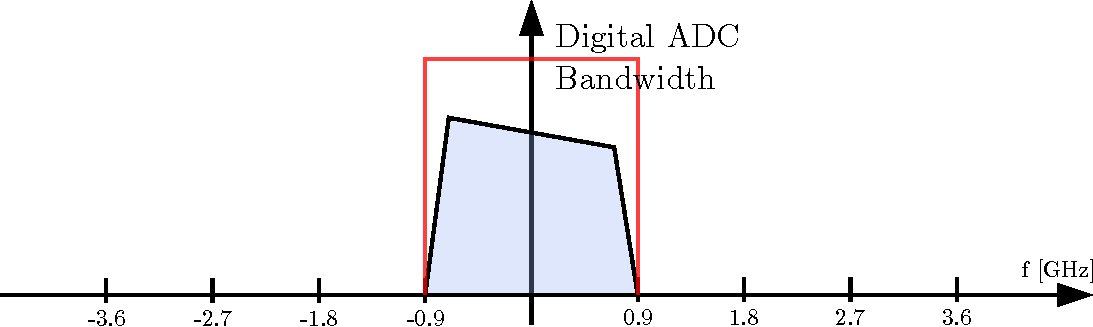
\includegraphics[width=0.8\textwidth]{figures/rx_0_freq_rx_if2}
    \caption{\gls{RX} low \gls{IF}}
    \label{fig:rx_0_freq_rx_if2}
  \end{subfigure}
  \caption{Quadrature Baseband Sampling Receiver in Frequency Domain}
  \label{fig:rx_0_freq}
\end{figure}

\subsection{Intermediate Frequency Sampling Receiver}
\label{sec:rx_1}
Next a different receiver architecture was considered which uses
$90^\circ$ couplers for image rejection as described in \secref{sec:rx_rf_1}
and than samples at an \gls{IF} aligned to the first Nyquist-zone as described
in \secref{sec:rx_adc_0}. \\

The block diagram is shown in \figref{fig:rx_1_bd}, the spectra in
\figref{fig:rx_1_freq} and the used frequencies in \tblref{tab:rx_1}. \\

The second \gls{IF} of $f_{\text{LO}_2} = 0.9$ was assigned, such that
the 1.8 GHz wide signal fully falls into the first Nyquist-zone of
a single \gls{ADC} sampling at 3.6 GHz. Again a \gls{DC}-block
is used in front of the \gls{ADC}. \\

The channel selection is done by a combination of two filter. First
a  high-pass filter (\figref{fig:rx_1_freq_rx_if1}) before
the second mixer removes signals between $f_{\text{RX LO}}$ and
$f_{\text{c}} - \frac{B}{2}$, including the strong \gls{TX} \gls{LO}
leakage. The low-pass filter on the lower \gls{IF}
(\figref{fig:rx_1_freq_rx_if2}) is the second part of the channel
selection filter by preventing aliasing. \\

A drawback of this architecture is, that it requires a single \gls{ADC}
at the symbol speed $f_{\text{symb}}$ instead of two \gls{ADC} channels at
$\frac{f_{\text{symb}}}{2}$ used by the two other architectures.
Such \gls{ADC} can, as it was done in our setup, be build using a two channel
\gls{ADC} in interleaved mode. This may introduce new errors as the not
perfect balancing of both channels and a high clock jitter frequency
component at $f_{s}$. \\

\begin{table}[h]
  \centering
  \begin{tabular}{|l|r@{}l@{~}l|}
    \hline
    $f_{\text{TX IF}}$ & 1&.7&GHz \\ \hline
    $f_{\text{TX LO}}$ & 58&.2&GHz \\ \hline
    $f_{\text{RX LO}}$ & 57&&GHz \\ \hline
    $f_{\text{RX IF}}$ & 2&.9&GHz \\ \hline
    $f_{\text{LO}_2} $ & 2&&GHz \\ \hline
    $f_c$           & 59&.9&GHz \\ \hline
    Signal Bandwidth B & 1&.8&GHz \\ \hline
    Number of \gls{ADC} Channels & 1&& \\ \hline
    Sample Rate $f_s$ & 3&.6&GHz \\ \hline
  \end{tabular}
  \caption{Properties of Intermediate Frequency Sampling Receiver}
  \label{tab:rx_1}
\end{table}

\begin{figure}[p]
  \centering
  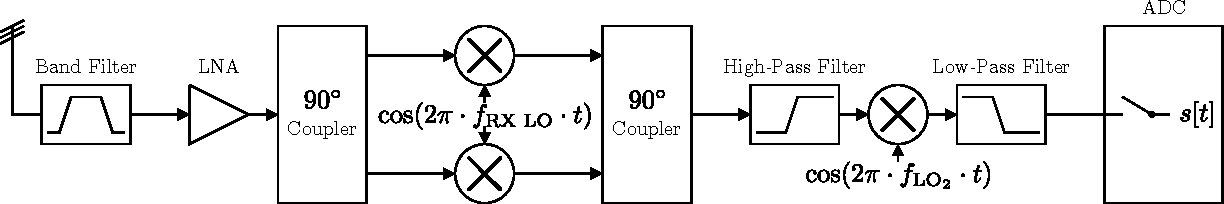
\includegraphics[width=\textwidth]{figures/rx_1_bd}
  \caption{Block Diagram of Intermediate Frequency Sampling Receiver}
  \label{fig:rx_1_bd}
\end{figure}

\begin{figure}[p]
  \centering
  \begin{subfigure}{\textwidth}
    \centering
    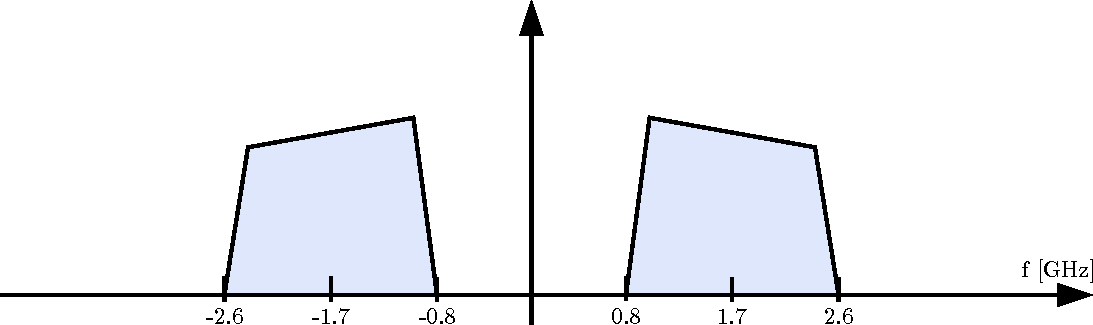
\includegraphics[width=0.8\textwidth]{figures/rx_1_freq_tx_if}
    \caption{\gls{TX} \gls{IF}}
    \label{fig:rx_1_frq_tx_if}
  \end{subfigure}
  \vspace{4ex} \\
  \begin{subfigure}{\textwidth}
    \centering
    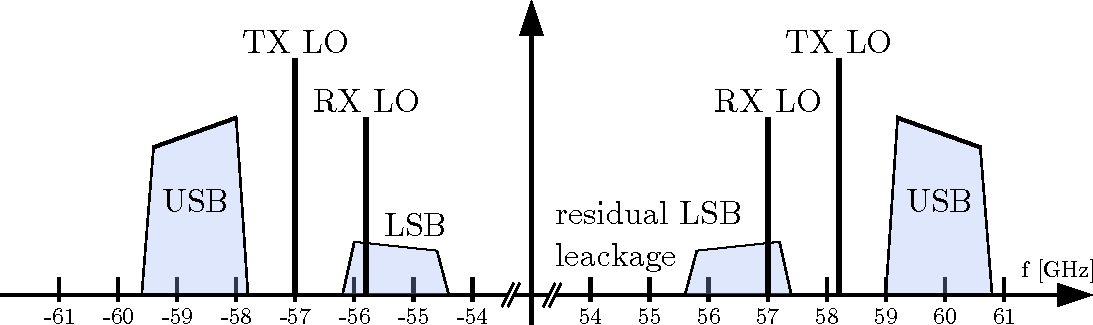
\includegraphics[width=0.8\textwidth]{figures/rx_1_freq_rf}
    \caption{\gls{RF}}
    \label{fig:rx_1_freq_rf}
  \end{subfigure}
  \vspace{4ex} \\
  \begin{subfigure}{\textwidth}
    \centering
    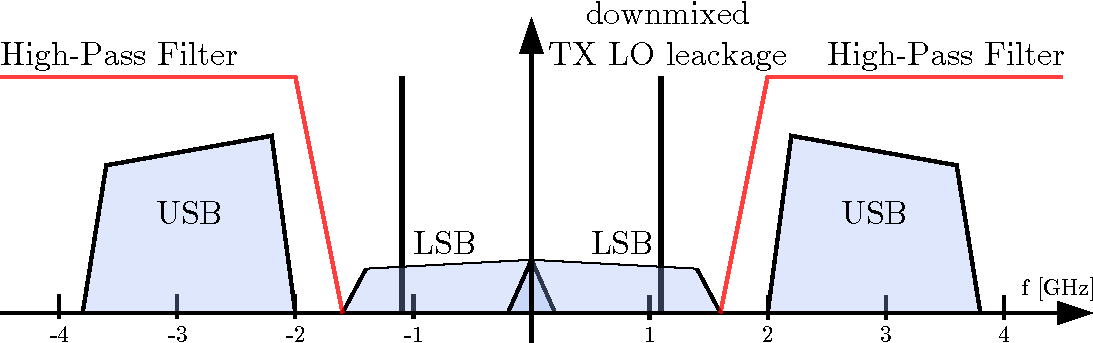
\includegraphics[width=0.8\textwidth]{figures/rx_1_freq_rx_if1}
    \caption{first (high) \gls{RX} \gls{IF}}
    \label{fig:rx_1_freq_rx_if1}
  \end{subfigure}
  \vspace{4ex} \\
  \begin{subfigure}{\textwidth}
    \centering
    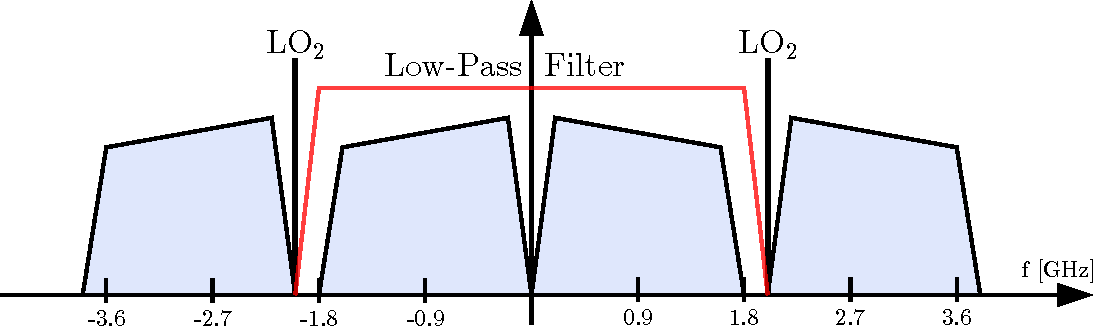
\includegraphics[width=0.8\textwidth]{figures/rx_1_freq_rx_if2}
    \caption{second (low) \gls{RX} \gls{IF}}
    \label{fig:rx_1_freq_rx_if2}
  \end{subfigure}
  \caption{Intermediate Frequency Sampling Receive in Frequency Domain}
  \label{fig:rx_1_freq}
\end{figure}

\subsection{Quadrature Intermediate Frequency Sub-Nyquist Sampling Receiver}
\label{sec:rx_2}
The third receiver architecture, which was used for most measurements,
was motivated by having only very few components that can add noise
and errors due to non-linear terms. \\

It is, however, based on the assumption that no other channels of the
60 GHz spectrum are used, except those, where we send residuals our self.
Therefor the very strong \gls{TX} \gls{LO} leakage and
the residual \gls{TX} \gls{LSBand} leakage are shown in all plots. \\

As shown in the block diagram in \figref{fig:rx_2_bd}, it only uses one
\gls{IF} and performs Quadrature Sub-Nyquist Sampling as described
in \secref{sec:rx_adc_2}. \\

Since the two mixers of the 58-63 GHz converter work at much
higher frequencies than those used in the other architectures, the
\gls{LO}-leakage and it's self-mixing is even more pronounced.
Because of that and probably also due to further component restrictions,
the converter is specified for an \gls{IF} of 1-5 GHz as noted in
\secref{sec:comp_sivers}.
Since the desired signal, which has a full bandwidth of 1.8 GHz,
results in an \gls{RX} \gls{IF} between 1.0 and 2.8 GHz, this just meets
this specifications. \\

The \gls{ADC} 12d1800 has an analog bandwidth of typically 2.8 GHz
as described in \secref{sec:comp_adc}.
Therefor the upper limit of the 2.8 GHz of \gls{RX} \gls{IF} meets this
requirement as well. \\

After the $f_{\text{RX IF}}$ is fully defined by this constraints, the
$f_{\text{TX LO}}$ and $f_{\text{RX LO}}$ have to be looked at.
As we can see in \figref{fig:rx_2_freq_a_0} the \gls{TX} \gls{LO}
leakage will be at $q = \pm \left(f_{\text{RX LO}} - f_{\text{TX LO}} \right)$.
To be optimally suppressed by the channel filter, this difference should be as
small as possible. On the other hand, the residual \gls{TX} \gls{LSBand} signal
will be separated from the desired \gls{TX} \gls{USBand} signal by $2 \cdot q$
which demands for $q \geq \frac{f_s}{2}$. \\
Unfortunately only one of this constraints can be meet. Since the \gls{TX}
\gls{LO} leakage is much stronger then the residual \gls{TX} \gls{LSBand}
leakage, the difference was chosen to be $q = 0.7 \;\text{GHz}$ resulting in the
\gls{TX} \gls{LO} leakage to be well suppressed by the channel filter while
the residual \gls{TX} \gls{LSBand} signal overlaps 0.6 GHz. \\

The absolute value of $f_{\text{RX LO}}$ was then chosen such that the
carrier frequency $f_c = 60.1 \text{GHz}$ is in the middle of the
converter's \gls{RF} specification and the residual \gls{TX} \gls{LSBand}
at 54.9 GHZ is well outside. \\

Consequently $f_{\text{TX IF}} = f_c - f_{\text{TX LO}} = 2.6 \;\text{GHz}$,
which meets the \gls{IF} specification of the converter as well. \\

The receiver first mixes the \gls{RF} signal $r(t)$ with a the local oscillator
at $f_{\text{RX LO}}$ and a $90^\circ$ shifted version of this oscillator.
Again the frequency components at $\pm (f_c + f_{\text{RX LO}})$ are
automatically filtered and noted as a low-pass filter LP.
See: Equations \eqref{eq:rx_2_a_0}, \eqref{eq:rx_2_a_1} as well as
\figref{fig:rx_adc_1_freq_cos}, \figref{fig:rx_adc_1_freq_sin},
\figref{fig:rx_2_freq_a_0} and \figref{fig:rx_2_freq_a_1} \\

\begin{subequations}
  \begin{alignat}{2}
    a_0(t) &= \text{LP}\{r(t) \cdot \cos(2\pi \cdot f_{\text{RX LO}} \cdot t)\}
    \label{eq:rx_2_a_0} \\
    a_1(t) &= \text{LP}\{r(t) \cdot \sin(2\pi \cdot f_{\text{RX LO}} \cdot t)\}
    \label{eq:rx_2_a_1}
  \end{alignat}
\end{subequations}

Next the channel filter, which is implemented as a band pass filter is applied.
The resulting signals $b_0(t) = \text{BP}\{a_0(t)\}$ and
$b_1(t) = \text{BP}\{a_1(t)\}$ are shown in \figref{fig:rx_2_freq_b_0}
and \figref{fig:rx_2_freq_b_1}. \\

Then the two analog signals $b_0(t)$ and $b_1(t)$ are sampled by two
separate \gls{ADC} channels as noted in \eqref{eq:rx_2_c_0} and
\eqref{eq:rx_2_c_1} and drawn in \figref{fig:rx_2_freq_c_0}
and \figref{fig:rx_2_freq_c_1}. \\

\begin{subequations}
  \begin{alignat}{2}
    c_0[k] &= \int_{-\infty}^{\infty}
    b_0(t) \cdot \delta\left(t - \frac{k}{f_s}\right) \; \text{d}t
    \;\; \forall k \in \mathbb{Z}
    \label{eq:rx_2_c_0} \\
    c_1[k] &= \int_{-\infty}^{\infty}
    b_1(t) \cdot \delta\left(t - \frac{k}{f_s}\right) \; \text{d}t
    \;\; \forall k \in \mathbb{Z}
    \label{eq:rx_2_c_1}
  \end{alignat}
\end{subequations}

Next the two digital signals $c_0[k]$ and $c_1[k]$ are interpreted as one
complex discrete signal $d[k] = c_1[k] + j \cdot c_0[k]$ as shown in
\figref{fig:rx_2_freq_d}. \\

To get a better picture of how the resulting signal looks like,
\figref{fig:rx_2_freq_e} shows $e[k] = -j \cdot d[k]$.
As noticed before, this architecture does not fully suppress neighbouring
channels. The signal originating from the \gls{TX} \gls{LSBand} residual is
colored yellow while to desired signal stays blue. \\

The get the correct baseband signal $f[k]$, $e[k]$ has to be shifted by
$f_{\text{RX IF}} - f_s = 100 \; \text{MHz}$:

\begin{align}
  f[k] = e[k] \cdot \exp\left(-2\pi \cdot j \cdot
  \frac{f_{\text{RX IF}} - f_s}{f_s} \cdot k \right)
  \;\; \forall k \in \mathbb{Z}
\end{align}

\begin{table}[h]
  \centering
  \begin{tabular}{|l|r@{}l@{~}l|}
    \hline
    $f_{\text{TX IF}}$ & 2&.6&GHz \\ \hline
    $f_{\text{TX LO}}$ & 57&.5&GHz \\ \hline
    $f_{\text{RX LO}}$ & 58&.2&GHz \\ \hline
    $f_{\text{RX IF}}$ & 1&.9&GHz \\ \hline
    $f_c$            & 60&.1&GHz \\ \hline
    Signal Bandwidth B & 1&.8&GHz \\ \hline
    Number of \gls{ADC} Channels & 2&& \\ \hline
    Sample Rate $f_s$ & 1&.8&GHz \\ \hline
  \end{tabular}
  \caption{Properties of Quadrature Intermediate Frequency
    Sub-Nyquist Sampling Receiver}
  \label{tab:rx_2}
\end{table}

\begin{figure}[p]
  \centering
  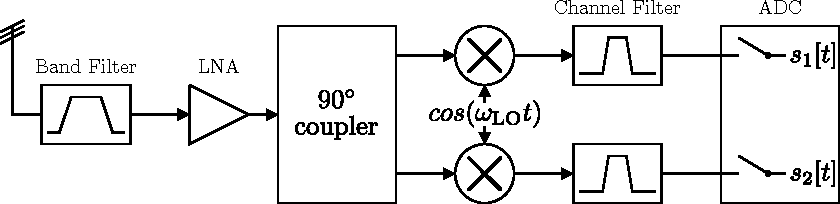
\includegraphics[width=\textwidth]{figures/quad_if_rx_block_diagram}
  \caption{Block Diagram of Quadrature Intermediate Frequency Sub-Nyquist Sampling Receiver}
  \label{fig:rx_2_bd}
\end{figure}

\begin{figure}[p]
  \centering
  \begin{subfigure}{0.45\textwidth}
    \centering
    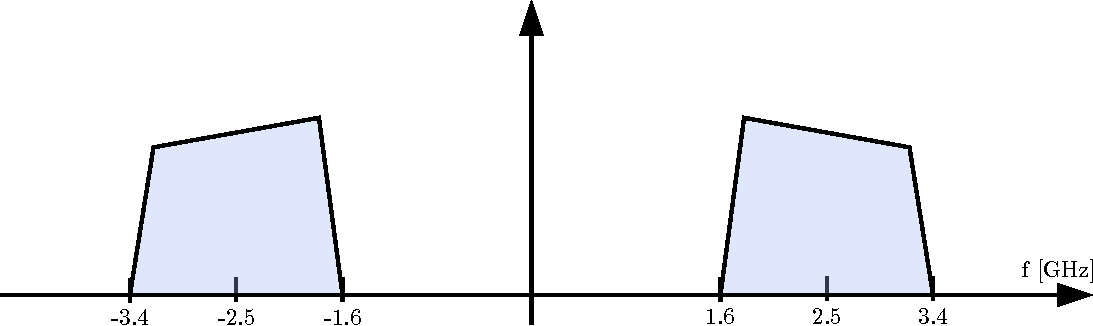
\includegraphics[width=\textwidth]{figures/rx_2_freq_tx_if}
    \caption{\gls{TX} \gls{IF}}
    \label{fig:rx_2_freq_tx_if}
  \end{subfigure}
  ~
  \begin{subfigure}{0.45\textwidth}
    \centering
    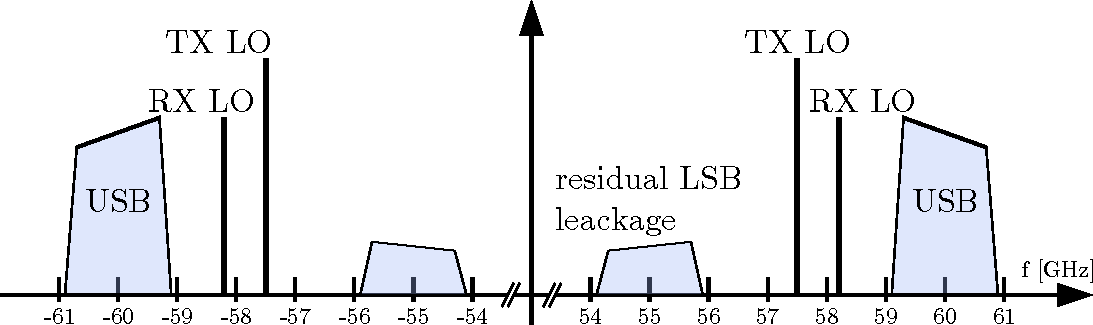
\includegraphics[width=\textwidth]{figures/rx_2_freq_rf}
    \caption{$r(t)$ : \gls{RF}}
    \label{fig:rx_2_freq_rf}
  \end{subfigure}
  \vspace{4ex} \\
  \begin{subfigure}{0.45\textwidth}
    \centering
    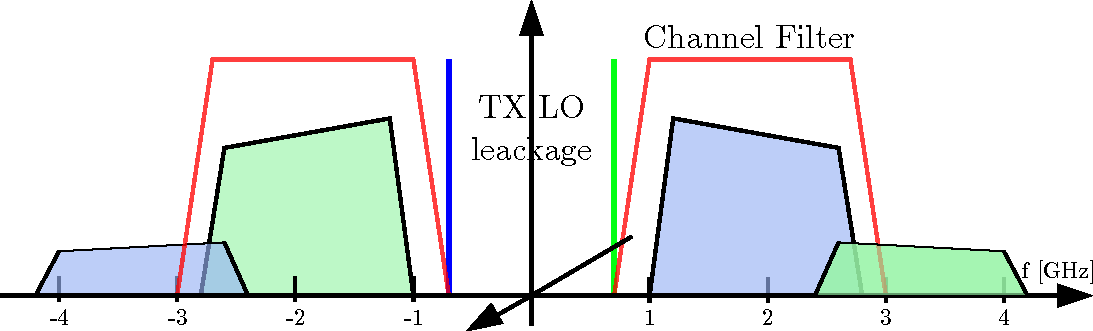
\includegraphics[width=\textwidth]{figures/rx_2_freq_a_0}
    \caption{$a_0(t) = \text{LP}\{r(t) \cdot \cos(2\pi \cdot f_{\text{RX LO}} \cdot t)\}$}
    \label{fig:rx_2_freq_a_0}
  \end{subfigure}
  ~
  \begin{subfigure}{0.45\textwidth}
    \centering
    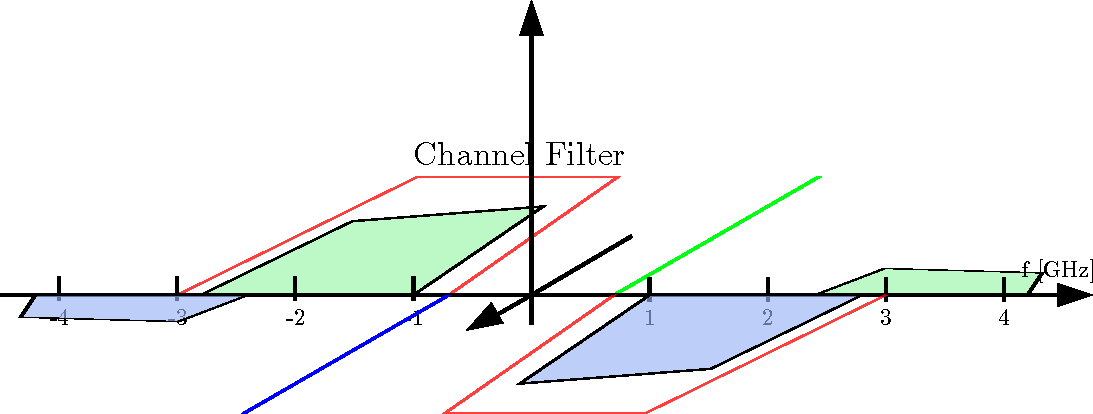
\includegraphics[width=\textwidth]{figures/rx_2_freq_a_1}
    \caption{$a_1(t) = \text{LP}\{r(t) \cdot \sin(2\pi \cdot f_{\text{RX LO}} \cdot t)\}$}
    \label{fig:rx_2_freq_a_1}
  \end{subfigure}
  \vspace{4ex} \\
  \begin{subfigure}{0.45\textwidth}
    \centering
    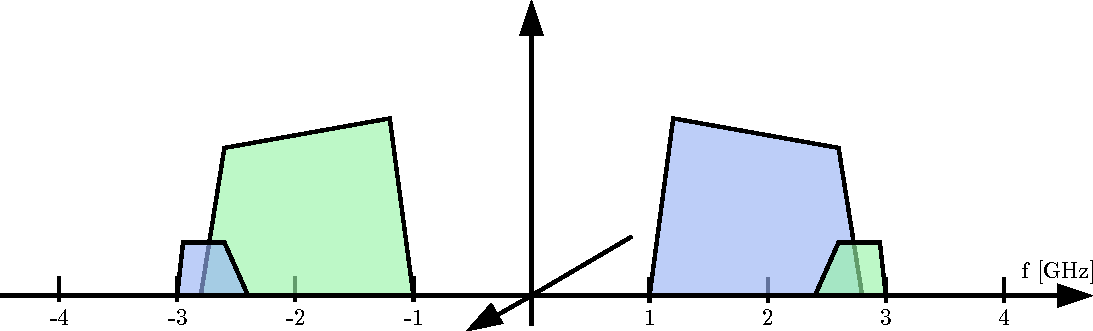
\includegraphics[width=\textwidth]{figures/rx_2_freq_b_0}
    \caption{$b_0(t) = \text{BP}\{a_0(t)\}$}
    \label{fig:rx_2_freq_b_0}
  \end{subfigure}
  ~
  \begin{subfigure}{0.45\textwidth}
    \centering
    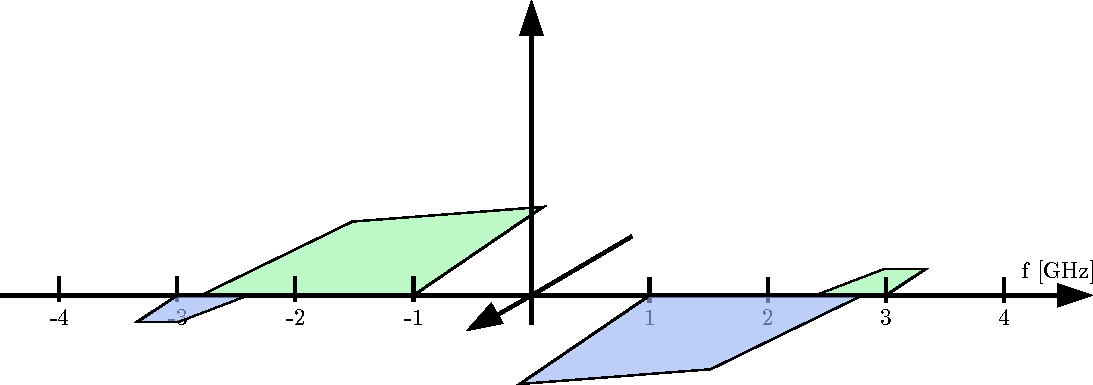
\includegraphics[width=\textwidth]{figures/rx_2_freq_b_1}
    \caption{$b_1(t) = \text{BP}\{a_1(t)\}$}
    \label{fig:rx_2_freq_b_1}
  \end{subfigure}
  \vspace{4ex} \\
  \begin{subfigure}{0.45\textwidth}
    \centering
    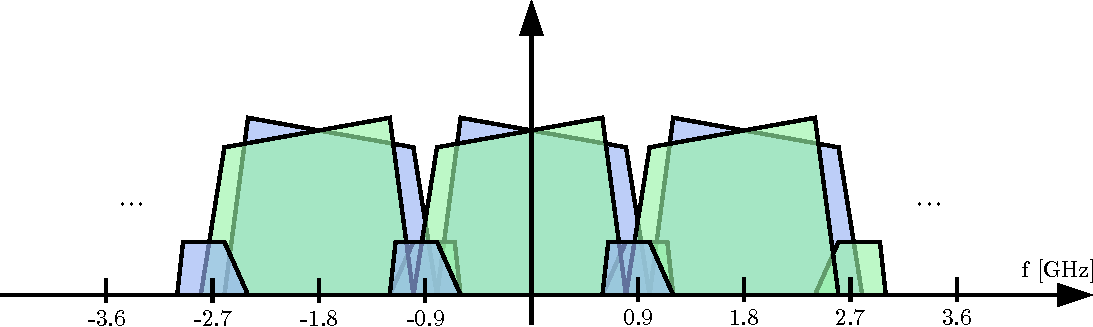
\includegraphics[width=\textwidth]{figures/rx_2_freq_c_0}
    \caption{$c_0[k] = b_0(k/f_s)$}
    \label{fig:rx_2_freq_c_0}
  \end{subfigure}
  ~
  \begin{subfigure}{0.45\textwidth}
    \centering
    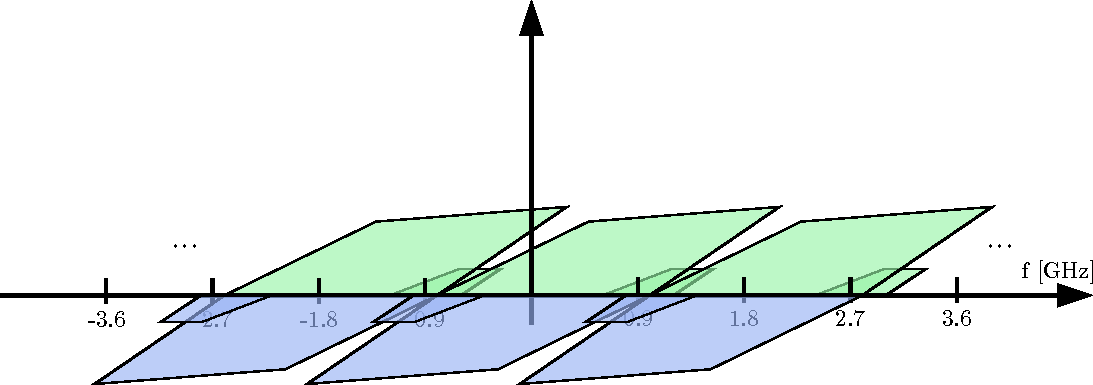
\includegraphics[width=\textwidth]{figures/rx_2_freq_c_1}
    \caption{$c_1[k] = b_1(k / f_s)$}
    \label{fig:rx_2_freq_c_1}
  \end{subfigure}
  \vspace{4ex} \\
  \begin{subfigure}{0.45\textwidth}
    \centering
    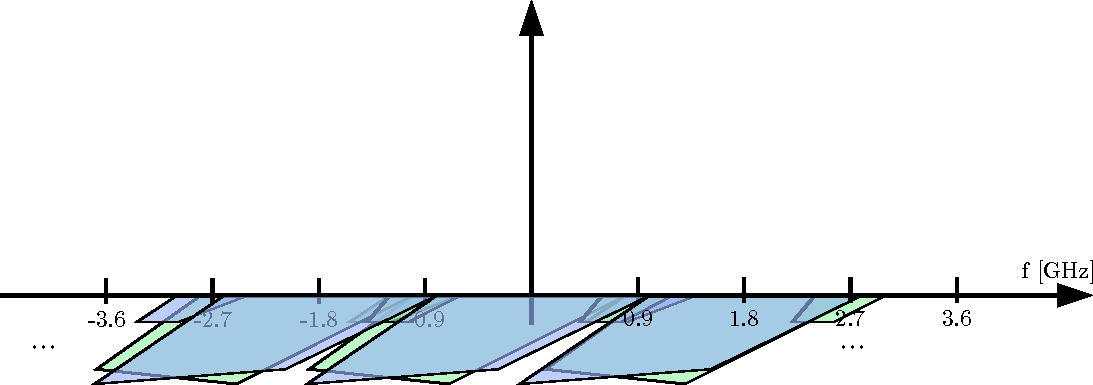
\includegraphics[width=\textwidth]{figures/rx_2_freq_jc0}
    \caption{$j \cdot c_0[k]$}
    \label{fig:rx_2_freq_jc0}
  \end{subfigure}
  ~
  \begin{subfigure}{0.45\textwidth}
    \centering
    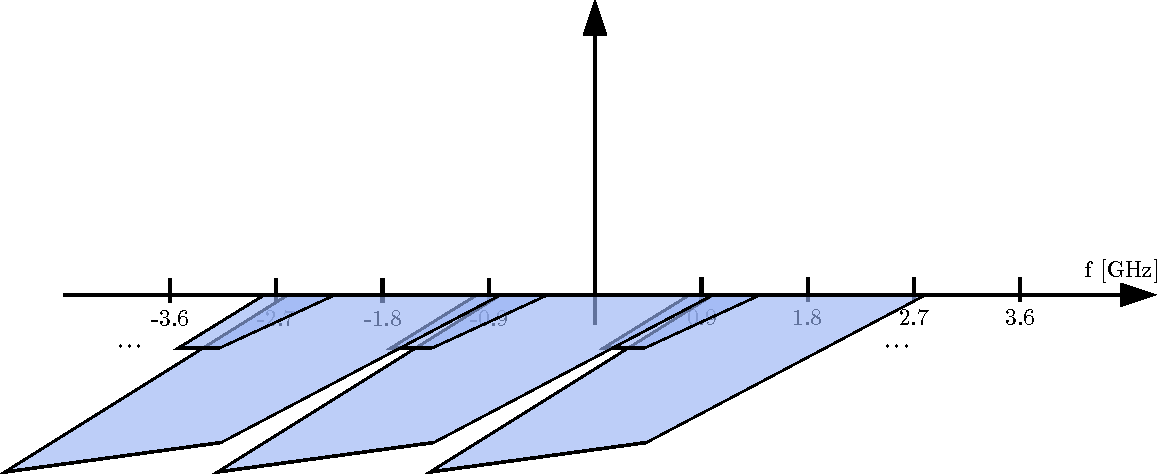
\includegraphics[width=\textwidth]{figures/rx_2_freq_d}
    \caption{$d[k] = c_1[k] + j \cdot c_0[k]$}
    \label{fig:rx_2_freq_d}
  \end{subfigure}
  \vspace{4ex} \\
  \begin{subfigure}{0.45\textwidth}
    \centering
    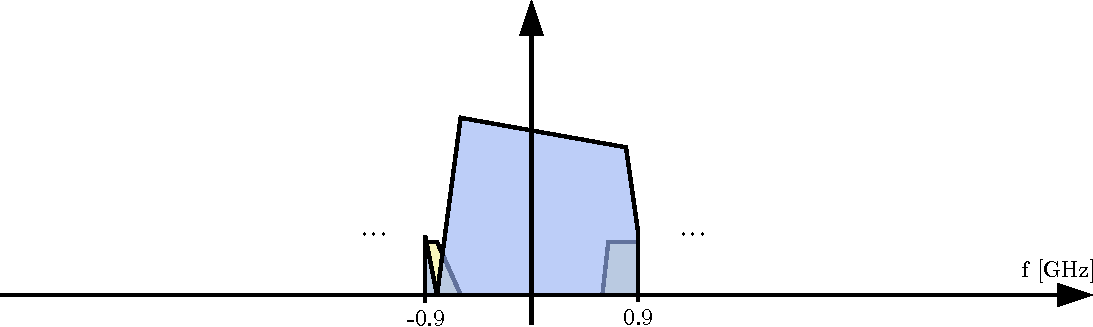
\includegraphics[width=\textwidth]{figures/rx_2_freq_e}
    \caption{$e[k] = -j \cdot d[k]$}
    \label{fig:rx_2_freq_e}
  \end{subfigure}
  \caption{Quadrature Intermediate Frequency Sub-Nyquist Sampling Receiver
    in Frequency Domain}
  \label{fig:rx_2_freq}
\end{figure}

%%  LocalWords:  Sivers IMA sivers USBand LSBand DAC coupler rx rf bd
%%  LocalWords:  interferer SNR LNA convolve Couplers couplers Hs Hb
%%  LocalWords:  hilbert Baseband baseband adc eq ja Nyquist Meca ISI
%%  LocalWords:  jitter nyquist
